\documentclass[a4paper, 12pt]{article}

\usepackage[left = 1.5cm,
            right = 1.5cm,
            top = 1.5cm,
            bottom = 1.5cm,
            footskip = 0cm]{geometry}
\usepackage{graphicx} % Required for inserting images
\usepackage{wrapfig}
\usepackage{listings}
\usepackage{xcolor}

\definecolor{codebackground}{rgb}{0.95,0.95,0.92} % Choisir une couleur de fond de code ici

\lstdefinestyle{mystyle}{
    language=C++,
    basicstyle=\scriptsize\ttfamily,
    frame=single,
    rulecolor=\color{black},
    backgroundcolor=\color{codebackground},
    lineskip={-1.5pt}
}

\lstset{style=mystyle}

\title{\textbf{Rapport pour le projet de INFOF202}}
\author{
    Ransy Lenny
    \and
    Lejeune Lucas
    }
\date{Janvier 2024}
\renewcommand*\contentsname{Table des matières}

\begin{document}
\setlength{\parindent}{0em}

\maketitle

Ce rapport vise a documenter le projet "Frogger" que nous avons réaliser. Nous traiterons les tâches que nous avons réalisées et comment nous les avons réalisées. Pour cela, nous parlerons des classes que nous avons codées pour faire ce projet, comment elles sont réparties dans le code et comment elles intéragissent entre elles. Nous justifierons aussi comment nous avons utilisé le modèle de conception MVC dans la partie jeu.

\tableofcontents

\pagebreak

\section{Résumé des tâches réalisées et fonctionnement du jeu}
% Résumer comment le jeu marche et listes les tâches réalisées
Nous avons réalisé les tâches principales et toutes les tâches additionnelles, sauf la tâches de l'éditeur de niveau. 
Ouvrons le jeu et voyons ce qui se passe. 
% Parler du fonctionnement du jeu quand tout sera fini

\section{Structure des fichiers: Utilisation du MVC}
% Parler de l'orga des fichiers

La structure des fichiers peut se diviser en plusieurs parties: les fichiers du jeu, ceux des menus, les mains et les images du jeu. \\

\begin{wrapfigure}{r}{3cm}
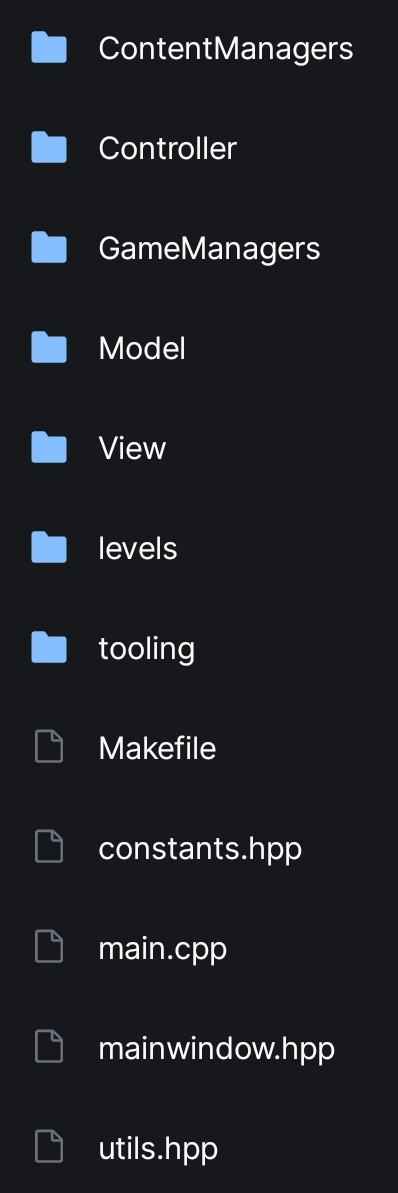
\includegraphics[width=3cm]{Images/folders.jpg}
\end{wrapfigure}

Le dossier \texttt{ContentManagers} contient tout les fichiers de code en rapport avec la gestion des menus du jeu.\\

Les dossiers \texttt{Controller}, \texttt{Model} et \texttt{View} contiennent le code parmettant de faire tourner le jeu (la partie plateau, qui ne compte pas le menu).
Cette disposition met en évidence l'utilisation du MVC. Prenons la gestion de la grenouille comme exemple. 
Les fichiers gérant les contrôles de celle-ci se trouvent dans le dossier \texttt{Controller}, ceux qui gèrent ses propriétés dans le plateau se trouvent dans \texttt{Model} et enfin, ceux qui gèrent son affichage se trouvent dans \texttt{View}. Tout le code de ces fichiers est utilisé dans les fichiers de \texttt{GameManagers} pour avoir un jeu fonctionnel.\\

Le dossier \texttt{levels} contient les données des niveaux sauvegardés en fichiers \texttt{.csv}, et les scores obtenus sur ceux-ci. Plus de détails seront donnés dans les chapitres concernés. \\

Le dossier \texttt{tooling} contient tout les outils construits grâce aux outils venant la librairie FLTK qui sont surtout utilisés dans la partie \texttt{View} et \texttt{ContentManagers}. \\

Le fichiers \texttt{constants.hpp} contient toutes les constantes utilisées dans le projet, comme par exemple la taille des bouttons dans le menu. \\

Enfin, les fichiers \texttt{main.cpp} et \texttt{mainwindow.hpp} s'occupent d'assembler toutes les classes et fonctions ensemble, pour obtenir l'application Frogger au complet. 

\section{Réalisation de la base du jeu (Tâches de base)}
% On parle du tout début juste avec les roadlanes
Bien sûr, pour cette tâche, la première chose à faite a été de faire un support pour utiliser fltk. C'est là que les fichiers \texttt{main.cpp} et \texttt{MainWindow.hpp} rentrent en jeu.

\subsection{Modèle}

Il nous faut maintenant un modèle fonctionnel. Le but est de d'abord faire un plateau de jeu. \\

Les rangées sont des objets de classe \texttt{Lane}, classe qui est définie dans le fichier \texttt{lanes.hpp}. La classe \texttt{BoardModel} contient alors un vecteur de pointeurs vers des objets \texttt{Lane}. Pour avoir différents types de rangées, il suffit alors de définir ces types grâce à de l'héritage sur la classe \texttt{Lane}. Nous définissons alors dans le fichier \texttt{lane.hpp} les classes \texttt{FinnishLane} (nous en parlons dans le chapitre \ref{lilies}), \texttt{SafeLane} et \texttt{RoadLane}. \\

La classe \texttt{SafeLane} représente une rangée basique sans aucun obstacle. La classe \texttt{RoadLane} est par contre un peu plus complexe. Nous voulons d'abord définir ce qu'est une voiture, ceci se passe dans le fichier \texttt{movingobjects.hpp}. Une voiture est un objet de classe \texttt{Car} qui contient quelques getters et une méthode \texttt{collide} qui servira à voir s'il y a une collision avec la grenouille. Cette classe hérite de la classe abstraite \texttt{MovingObject}. Cela nous permet de créer une classe abstraite appelée \texttt{MovingObjectLane} qui hérite de \texttt{Lane} et qui possède en instance un vecteur de pointeurs vers des objets de classe \texttt{MovingObject}. Cette classe possède une méthode qui permet de regarder s'il y a collision entre la grenouille et au moins un objet. La classe \texttt{RoadLane} est alors juste un successeur de la classe \texttt{MovingObjectLane}. \\

Toutes les classes et méthodes sont après assemblées dans la classe \texttt{BaordModel} pour faire un plateau fonctionnel.

Parlons maintenant de la grenouille. Elle sera définie par un objet de classe \texttt{Frog}, classe qui est définie dans le fichier \texttt{frog.hpp}. Les collisions entre celle-ci et les objets sont gérées par les objets qui possèdent des méthodes qui prennent un référence vers la grenouille en paramêtre. La classe \texttt{Frog} possède alors un getter vers la rangée à laquelle elle se trouve, et un autre vers sa position x (en pixels). Cette classe possède tout de même une méthode \texttt{inBaord} qui vérifie si la grenouille ne sort pas du plateau. C'est aussi dans cette classe que sont gérés la mort, mais nous parlerons de cela dans le chapitre \ref{lives}. L'utilité des autres méthodes de cette classe sera abordée plus tard.

\subsection{Controlleur}

Les contrôles de la grenouille se passent dans la classe \texttt{Controller} qui se trouve quand le fichier \texttt{controller.hpp} qui est contenu dans le dossier \texttt{Controller}.
La classe \texttt{Frog} possède déjà des méthodes permettant de changer sa position sur le plateau, il faut alors juste les utiliser quand nous appuyons sur une touche. La méthode \texttt{processKey} sert à gérer ces actions. Les contrôles se font avec les touches zqsd comme pour beaucoup de jeux. 

\subsection{Vue}

Tout ce dont nous allons parler dans ce sous-chapitre se passe dans le dossier \texttt{View}. Pour résumer, pour presque chaque classe de la partie modèle, il y a une classe de la partie vue qui s'occupe de l'affichage de ce modèle. \\

D'abord, nous avons un fichier \texttt{movingobjectview.hpp} qui contient la classe \texttt{CarView} qui hérite de la classe \texttt{MovingObjectView}. L'intérêt de ces classes est de pouvoir utiliser la méthode \texttt{draw} pour afficher l'objet sur la plateau. Les couleurs sont choisies dans le constructeur et les tailles sont données par l'objet de classe \texttt{MovingObject} qu'elle prennent en paramêtre dans le constructeur. \\

Ensuite, nous avons un fichier \texttt{laneview.hpp} qui possède la classe abstraite \texttt{LaneView} et les classes héritantes \texttt{SafeLaneView}, \texttt{FinishLaneView} et \texttt{RoadLaneView}. Leur intérêt est aussi de pouvoir utiliser la méthode draw pour les afficher sur le plateau. La classe \texttt{RoadLaneView} possède en plus un vecteur de pointeurs vers des objets de type \texttt{CarView} pour pouvoir dessiner les voitures sur les rangées concernées. La méthode \texttt{draw} de \texttt{CarView} est alors appelée dans la méthode \texttt{draw} de \texttt{RoadLaneView}. \\

Nous parlerons de l'affichage de la grenouille dans les chapitres \ref{lives} et \ref{frogview}

Enfin, à l'aide de toutes ces méthodes \texttt{draw} (il y en a aussi une pour la grenouille, nous pouvons créer une classe \texttt{BoardView} dans le fichier \texttt{boardview.hpp} contenant une méthode \texttt{draw} elle même et qui va dessiner le plateau selon l'instance de classe \texttt{BoardModel} (sous forme de pointeur) qui lui sera donnée.

\subsection{Assemblage pour faire un jeu fonctionnel}

Il nous faut maintenant assembler le tout pour faire un plateau fonctionnel. Ceci se fait dans le dossier \texttt{GameManagers}, et plus particulièrement dans le fichier \texttt{gameloop.hpp}. Dans celui-ci se trouve la classe \texttt{GameLoop} prennant tout ce que nous avons défini (et d'autres éléments dont nous parlerons plus tard) en instance. Le plateau s'initialise alors avec le constructeur, et s'anime en exécutant à chaque frame la méthode \texttt{update}. Nous verrons plus tard où cette méthode est exécutée. \\

\begin{lstlisting}
class GameLoop {
    private:
        std::shared_ptr<BoardModel> bm;
        std::shared_ptr<BoardView> bv;
        std::shared_ptr<FrogView> fv;
        std::shared_ptr<Frog> frog;
        std::shared_ptr<Score> score;
        std::shared_ptr<ScoreView> sv;
        std::shared_ptr<Controller> c;
        std::unique_ptr<ScoreSaver> ssv;
        std::shared_ptr<Score> best_score;
        std::unique_ptr<ScoreView> bs_show;
    public:
        GameLoop(unsigned int lvl);
        void update();
        std::shared_ptr<BoardModel> getModel();
        std::shared_ptr<BoardView> getView();
        std::shared_ptr<FrogView> getFrog();
        ~GameLoop() {}
};
\end{lstlisting}

\section{Réalisation des tâches additionnelles}
Maintenant que les tâches principales sont réalisées et que nous avons une bonne base, nous pouvons implémenter les fonctionnalités supplémentaires. 

\subsection{Rangées d'eau, buches et tortues} \label{turtle_class}

\underline{\textbf{Modèle:}} \\
Dans le fichier \texttt{movingobjects.hpp}, nous implémentons les tortues et les buches. Les collisions ne seront pas gérée de la même manière que pour les voitures, donc nous faisons un override. Nous parlerons plus en détail des méthodes de la classe \texttt{Turtle} dans le chapitre \ref{diving_turtles}. \\

\begin{lstlisting}
class Turtle: public MovingObject {
    private:
        bool diving;
    public:
        Turtle(int speed, const unsigned int head, const unsigned int size
                , const unsigned lane_id);
        void dive() final override;
        void undive() final override;
        bool isDiving() const final override;
        bool collide(Frog& frog) final override;
        ~Turtle() {}
};
\end{lstlisting}

\begin{lstlisting}
class Log: public MovingObject {
    public:
        Log(int speed, unsigned int head, const unsigned int size,
            const unsigned lane_id);
        bool collide(Frog& frog) final override;
        ~Log() {}
};
\end{lstlisting} \hspace{0.5cm}

Dans le fichier \texttt{lane.hpp}, nous implémentons deux nouvelles classes héritantes de \texttt{MovingObjectLane}. 
Nous parlerons aussi plus tard des méthodes de la classe \texttt{TurtleLane}. \\

\begin{lstlisting}
class LogLane: public MovingObjectLane {
    public:
        LogLane(const unsigned int id_num, const unsigned int& log_by_pack,
                const unsigned int& space_between_logs,
                const unsigned& space_between_packs,
                const int& first_log_placement,
                const unsigned int& size_log, const int& speed=0);
        bool water_lane() const override { return 1; }
        void handle_after_collision(Frog& frog) override;
        std::vector<std::shared_ptr<Log>> getLogs() const;
        ~LogLane() {}
};
\end{lstlisting}

\begin{lstlisting}
class TurtleLane: public MovingObjectLane {
    unsigned int turtle_by_pack;
    unsigned int diving_pack_id;
    bool is_diving = true;
    unsigned int diving_time;   // In frames
    unsigned int undiving_time;
    unsigned int diving_count = 0;
    public:
        TurtleLane(const unsigned int id_num
                   , const unsigned int& turtle_by_pack
                   , const unsigned int& space_between_turtles
                   , const unsigned& space_between_packs
                   , const int& first_turtle_placement
                   , const unsigned int& size_turtle
                   , const int& speed=1
                   , const unsigned int diving_pack_id = 0
                   , const unsigned int diving_time = 180
                   , const unsigned int undiving_time = 180);
        std::vector<std::shared_ptr<Turtle>> getTurtles() const;
        void handle_after_collision(Frog& frog) override;
        bool water_lane() const override { return 1; }
        void pack_dive();
        void pack_undive();
        void dive_update() final override;
        ~TurtleLane() {}
};
\end{lstlisting} \hspace{0.5cm}

% Parler des mouvements de la grenouille quand sur ces objets

\underline{\textbf{Vue:}} \\
Les implémentations gérant la vue de ces deux nouvelles rangées est similaire que pour celle des rangées de voitures. \\
\begin{lstlisting}
class LogView: public MovingObjectView {
    public:
        LogView(std::shared_ptr<Log> l);
        ~LogView() {}
};
\end{lstlisting}

\begin{lstlisting}
class TurtleView: public MovingObjectView {
    public:
        TurtleView(std::shared_ptr<Turtle> t);
        void draw() final override;
        ~TurtleView() {}
};
\end{lstlisting}

\subsection{Nénuphars} \label{lilies}

Dans le fichier \texttt{Model/waterlilies.hpp}, nous définissons une nouvelle classe \texttt{WaterLilies} qui va représenter les nénuphars. \\

\begin{lstlisting}
class WaterLilies {
    private:
        int x;
        bool visited=false;
    public:
        WaterLilies(int x);
        int getX();
        bool collide(Frog& frog);
        bool hasBeenVisited();
        void visit();
        ~WaterLilies() {}
};
\end{lstlisting} \hspace{0.5cm}

Nous pouvons maintenant parler de l'implémentation de la classe \texttt{FinishLane}. \\

\begin{lstlisting}
class FinishLane: public Lane {
    private:
        std::vector<std::shared_ptr<WaterLilies>> lilies;
    public:
        FinishLane(const unsigned int id);
        std::vector<std::shared_ptr<WaterLilies>> getLilies();
        ~FinishLane() {}
};
\end{lstlisting} \hspace{0.5cm}

La rangée de fin contient des nénuphars. Si la grenouille se trouve sur un nénuphar, elle y reste et une nouvelle grenouille apparait, mais ceci n'est que ce que le joueur voir. En réalité, nous affichons juste une grenouille sur le nénuphar, mais nous gardons la même grenouille tout le long de la partie. Nous la téléportons juste à a case départ à chaque fois qu'elle touche un nénuphar. Si tout les nénuphars sont remplis, alors un écran de victoire s'affiche. Ceci se fait en utilisant la classe \texttt{FullScreenJPEGImage} du fichier \texttt{tooling/image\textunderscore classes.hpp} et en utilisant l'image \texttt{imgs/won.jpeg}. Ces actions se passent dans la méthode \texttt{GameLoop::update()}.

\subsection{Vies de la grenouille} \label{lives}

Les vies de la grenouille sont représentées par l'instance \texttt{lives} de la classe \texttt{Frog}. A chaque exécution de 
\texttt{GameLoop::update()}, on regarde si la grenouille respecte une des conditions pour perdre une vie. Si oui, alors on décrémente \texttt{lives} avec la méthode \texttt{kill()}. Si \texttt{lives} est à 0, alors on affiche un écran de défaite de la même manière que nous l'avons fait avec la victoire (avec le fichier \texttt{imgs/lose.jpeg}. \\

La classe \texttt{FrogView} s'occupe de dessiner tout ce qui est relié à la grenouille. Nous parlons ici seulement des vies, le reste sera abordé dans le chapitre \ref{frogview}. La méthode \texttt{showLives()} est alors appelée dans la méthode \texttt{draw()}. \\

\begin{lstlisting}
class FrogView {    
    std::shared_ptr<Frog> frog;
    JPEGDrawer current_image{paths::frog_north_jpeg, frog->getX(),
                                static_cast<int>(frog->getLane()), HEIGHT, WIDTH};
public:
    FrogView(std::shared_ptr<Frog> f);
    void showLives();
    void draw();
};
\end{lstlisting}

\subsection{Tortues plongeantes} \label{diving_turtles}

Dans le modèle, une tortue plonge si son instance \texttt{diving} est à \texttt{True} (voir \ref{turtle_class}). Ce statut change surtout le comportement des collisions avec les tortues dans le modèle. Nous ordonnons à la tortue de plonger avec les méthodes \texttt{dive()} et \texttt{undive()}. Ces ordres sont alors données dans la classe \texttt{TurtleLane} (voir \ref{turtle_class}). Comme dans le jeu orginal, nous faisons plonger les tortues par paquets. Nous pouvons choisir les intervalles de temps entre la plongée et la remontée des tortues d'un paquet d'une rangée dans les paramêtres du constructeur de la classe. Nous pouvons aussi choisir quel paquet va plonger dans les paramêtres. La méthode \texttt{dive\textunderscore update()} va alors se charger de faire plonger et remonter les tortues en boucle avec les paramêtres choisis. Cette méthode est exécutée à chaque frame dans la méthode \texttt{GameLoop::update()}. \\

Nous changons forcément commment est affichée la tortue quand elle plonge. Pour cela, nous faisons en sorte que la méthode \texttt{TurtleView::draw()} ne marche que quand la tortue est à la surface.

\subsection{Directions de la grenouille} \label{frogview}
Les directions sont gérées avec l'enum class suivant:
\begin{lstlisting}
enum class FrogDirection {
    North, South, East, West
};
\end{lstlisting}
\subsection{Score}
\begin{lstlisting}
class Score {
    private:
        unsigned the_score = 0;
        int max_lane = 0;
    public:
        Score() = default;
        Score(unsigned score): the_score(score) {}

        void reachedWaterlily();
        void update(int new_lane_id);
        unsigned getScore() const;
        void resetBestLane();

        friend bool operator<(Score const& s1, Score const& s2);
        friend bool operator>(Score const& s1, Score const& s2);
        friend bool operator==(Score const& s1, Score const& s2);
        ~Score() = default;
};
\end{lstlisting}
\subsection{Meilleur score}

\subsection{Gestion des menus et écran d'accueil}

\subsection{Niveaux et sélection de niveau}

\subsection{Vies}


\end{document}
